\section{System Overview}
\label{sec:overview}

\subsection{Software-Defined Peripheral Subsystem}

\sys presents a logical PCIe hierarchy to the DUT. A logical endpoint has a
virtual BDF, configuration image, BAR routes, interrupt state, and a binding to
a backend. The backend may be a physical function attached to the FPGA host or
reachable through a remote transport. The DUT names only logical resources; it
does not know the host BDF, transport endpoint, or host-side DMA aperture.

Figure~\ref{fig:overview} maps the logical device contract onto the FPGA,
host coordinator, and physical backends. Four mechanisms realize this mapping:
logical topology construction, configuration-space virtualization, endpoint
semantic mediation, and DMA-path realization. The first two determine what the
DUT sees; the latter two make that device operational.

\begin{figure*}[t]
    \centering
    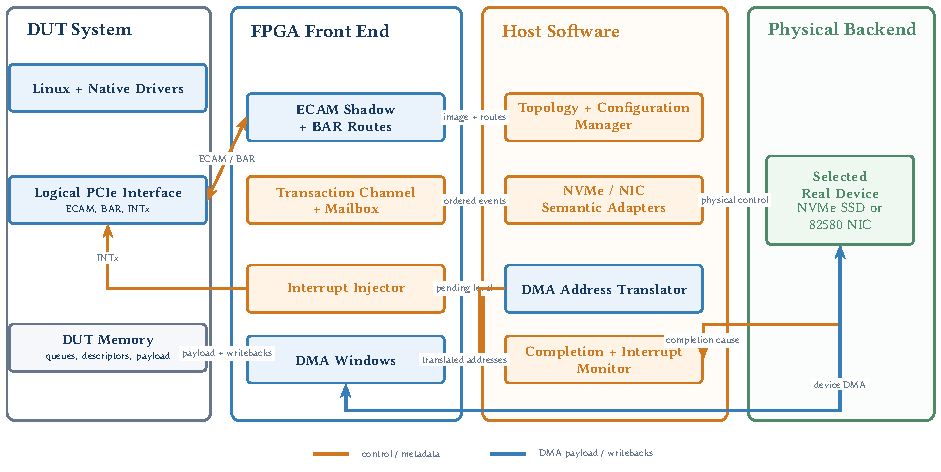
\includegraphics[width=\textwidth]{figures/system_architecture.pdf}
    \caption{\sys architecture. The DUT accesses a logical PCIe interface
    implemented by generic FPGA mechanisms. Host software owns topology and
    device semantics, while a selected physical backend executes device
    operations. Orange arrows carry control and metadata; blue arrows carry DMA
    payload and writebacks without traversing the semantic event channel.}
    \label{fig:overview}
    \Description{A DUT connects through a generic FPGA front-end to host
    coordination software and a real NVMe or Ethernet backend. Control and DMA
    paths are shown separately.}
\end{figure*}

\subsection{Three Planes and the SDN Analogy}
\label{sec:planes}

The architecture separates three responsibilities, following the distinction
between applications, control, and forwarding in software-defined networking
(SDN)~\cite{onf2014architecture}. In \sys, the \emph{software plane} is the
DUT's OS and native drivers, which consume a device interface. The
\emph{control plane} constructs that interface, binds logical endpoints to
backends, and mediates configuration and device control. Its mechanisms span
the FPGA front-end and host coordinator. The \emph{data plane} comprises the
physical backends and the paths through which they exchange payload with DUT
memory. These are functional responsibilities, not three physical machines;
host software in the control plane is distinct from DUT software in the
software plane.

\begin{figure*}[t]
    \centering
    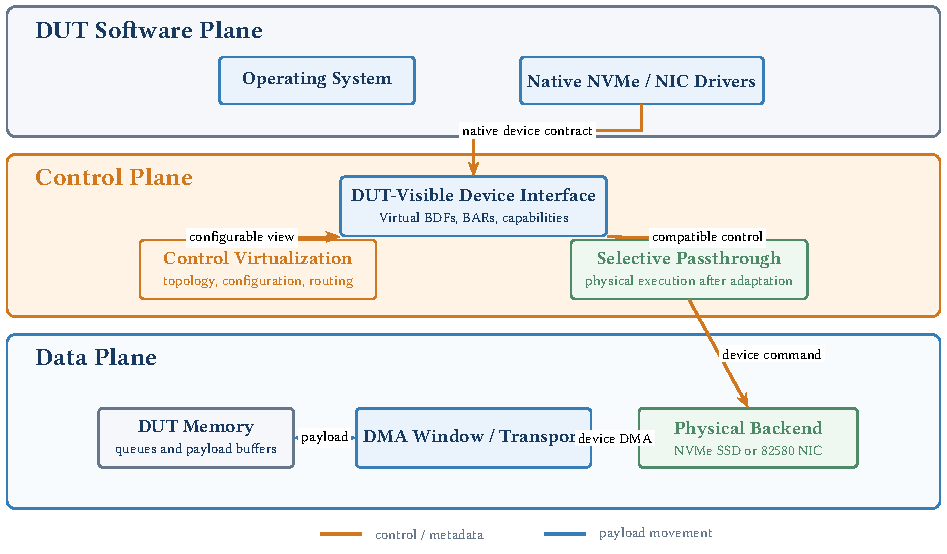
\includegraphics[width=0.92\textwidth]{figures/three_planes.pdf}
    \caption{SDN-inspired separation of peripheral access. Control
    virtualization makes the logical view and binding configurable, while
    selective passthrough retains execution by a physical backend after required
    adaptation. Payload movement follows an independently realized data path.
    Physical execution improves behavioral fidelity for the exposed operations,
    but does not imply direct-attachment timing or PCIe link fidelity.}
    \label{fig:planes}
    \Description{The DUT software plane consumes a virtual device interface.
    The control plane combines virtualization with selective passthrough. The
    data plane connects DUT memory to a real NVMe or Ethernet backend.}
\end{figure*}

The SDN analogy concerns programmable control over a separately realized data
path. The DUT software plane plays the role of a service consumer, but its
interface remains a native device protocol rather than an SDN application API.
The analogy also has a limit: a device submission refers to queues, DMA buffers,
and ownership transitions. Routing an access to the correct backend is
insufficient unless these stateful dependencies remain coherent.

Within the control plane, \emph{control virtualization} creates the logical
configuration and mediates state that differs from the physical backend.
\emph{Control passthrough} retains physical execution of compatible operations,
after any required address or protocol adaptation. The two responsibilities
can coexist for one endpoint. Here passthrough denotes use of the real device,
not transparent forwarding of every register access or full PCIe function
assignment. A direct DMA path is a separate choice: payload can bypass the
software proxy even when submission control is mediated.

\subsection{Dual Decoupling}

Table~\ref{tab:decoupling} separates the two mechanisms. Decoupling device
presentation from backend implementation answers \emph{what device does the DUT see
and which backend implements it?} Control-semantics--data-path decoupling
answers \emph{which operations require semantic mediation and how do payload
bytes move?} Neither alone is sufficient. The first without the second creates
a configurable view whose software proxy may become the data bottleneck. The
second without the first accelerates transfer but leaves device identity and
placement fixed.
The three planes identify responsibilities, whereas dual decoupling identifies
the architectural freedoms between them. The coherence rules below constrain
both freedoms.

\begin{table}[t]
\centering
\caption{Dual decoupling realizes the software-defined abstraction.}
\label{tab:decoupling}
\small
\begin{tabular}{@{}p{0.29\columnwidth}p{0.31\columnwidth}p{0.31\columnwidth}@{}}
\toprule
Mechanism & Separates & Enables \\
\midrule
Device presentation--backend implementation & DUT-visible PCIe identity and behavior from backend placement/realization & Endpoint rebinding, location transparency, software-selected composition \\
Control semantics--data path & Configuration and device control semantics from bulk payload movement & Programmable mediation with independently optimized DMA paths \\
\bottomrule
\end{tabular}
\end{table}

\subsection{Coherence after Separation}

Dual decoupling distributes one device contract across the DUT, FPGA, host
software, and physical backend. \sys restores a single observable order with
three invariants:
\begin{description}[leftmargin=*,style=nextline]
    \item[Configuration--route coherence.] A configuration write completes only
    after the authoritative image and any affected BAR route agree.
    \item[Submission--DMA coherence.] A physical doorbell is issued only after
    the submitted descriptor is stable and every device-visible address has
    been translated to a reachable target.
    \item[Data--completion coherence.] The DUT observes completion state or an
    interrupt only after the corresponding data is visible in DUT memory.
\end{description}
These invariants are not a third decoupling. They constrain the freedom created
by the two separations so the native driver still observes a legal device.

\subsection{Scope of Software Configuration}

The prototype supports a fixed maximum hierarchy and a finite set of generic
route entries. Software activates endpoints, chooses their types, assigns BDFs
under the provisioned switch ports, and binds backends before DUT enumeration.
This is software-configurable composition, not arbitrary online topology
rewiring or PCIe hotplug.

\begin{table}[t]
\centering
\caption{Longer-term access space and the slice evaluated in this paper.}
\label{tab:access-space}
\small
\begin{tabular}{@{}lll@{}}
\toprule
Dimension & Design space & Evaluated slice \\
\midrule
DUT stage & Pre-silicon / post-silicon & Pre-silicon \\
Software access & User / kernel / virtualized & Standard kernel driver \\
Backend placement & Local / remote & Local and host-remote \\
\bottomrule
\end{tabular}
\end{table}

The three dimensions motivate a $2\times3\times2$ design space, but they are
not independent features that the current prototype already implements in all
combinations. We use the table to state the intended abstraction boundary and
the evaluated slice precisely.
